\section{Introduction} \label{sec:introduction}

Recent advances cellular automata have established rich frameworks for continuous-valued state spaces with flexible rule sets.
The Lenia project is particularly notable for the rich taxonomy of emergent behaviors that have been systematically and extensively characterized \citep{chan2020lenia,horibe2023exploring}.

Notable developments have also been made in incorporating differentiable frameworks to enable rule set development using gradient descent \citep{mordvintsev2020growing,hamon2022learning}.
Other approaches to discovering rule sets include evolutionary computation \citep{jain2024capturing}, quality-diversity search \citep{faldor2024toward}, and sampling from the representation space of LLMs (e.g., LLMs, computer vision, etc.) \citep{kumar2024automating}.
Rule sets may also be spatially localized within a cellular automata model and allowed to evolve in tandem with the state dynamics they enact within simulation \citep{plantec2023flowlenia}.

Pertinent references for cellular automata work within the realm of artificial life include,
\begin{enumerate}
\item Moveable Feast Machine \citep{ackley2023robust,ackley2019building,ackley2012movable},
\item Lenia \citep{chan2020lenia,chan2019lenia},
\item differentiable Lenia \citep{hamon2022learning},
\item particle Lenia \citep{mordvintsev2022particle},
\item flow Lenia \citep{plantec2023flowlenia},
\item neural cellular automata \citep{mordvintsev2020growing},
\item self-replicating neural cellular automata \citep{sinapayen2023selfreplication},
\item discretized differentiable cellular automata \citep{miotti2025differentiable}, and
\item earlier works include CAPOW \citep{griffeath2003new}, Larger than Life \citep{evans2001larger}, RealLife \citep{pivato2007reallife}, and SmoothLife \citep{rafler2011generalization}.
\end{enumerate}
In other areas of biological research, cellular automata approaches have also been applied in modeling physiological \citep{peak2004evidence,davidenko1992stationary}, ecological \citep{breckling2011cellular}, and social \citep{beltran2009forecasting} processes.

Although a major goal of work with cellular automata is as a platform to study eco-evolutionary processes, a key epistimological distinction of cellular automata approaches is that no explicit self-replicating unit is defined \citep{hamon2022learning}; rather, interest lies in propagation of self-stabilizing ``soliton'' patterns in state space \citep{chan2019lenia}.
This enactivist approach is in contrast to agent-based, ``digital evolution'' approaches where an explicit self-replicating unit \citep{pennock2007models}.
Whereas such may be trivially tracked and characterized, implicit individuality introduces substantial challenges in tracking and characterizing eco-evolutionary dynamics within a simulation.

Another major benefit of cellular automata is that the spatial locality of update rules is well-suited to highly-distributed processing \citep{ackley2023robust}.
Lenia, in particular, uses a local update rule based on element-wise convolution using fixed-size kernels.
Figure \ref{fig:lenia-pseudocode} provides pseudocode for the Lenia update function.
A nice visual overview can be found at \url{https://developmentalsystems.org/sensorimotor-lenia/public/leniaVid.mp4}.



It is not hard to imagine how 2D or 3D lattice-based cellular automata with local update rules might effectively harness fabric-based hardware architectures such as the Cerebras Wafer-Scale Engine.
In fact, the Cerebras Software Development Kit (SDK) materials include an example implementation of Conway's Game of Life included with \citep{cerebras2024gol}.
Lenia, in particular, may potentially be compatible with an existing Field Equation modeling framework for the Wafer-Scale Engine \citep{woo2022disruptive}, which provides a higher-level, NumPy-like interface for programming on the Wafer-Scale Engine.
(Documentation for this project is hosted at \url{https://dirk-netl.github.io/WSE_FE/index.html}.)
Cerebras provides a PyTorch back-end, which may be useful for working with neural Cellular Automata \citep{cerebras2022pytorch}.
Fortuitously, reference code for differentiable Lenia used in prototype work for this project is implented in PyTorch \citep{hamon2022learning}.

Past work with agent-based simulations on the Cerebras Wafer-Scale engine have successfully applied hereditary stratrigtaphy methodology for decentralized phylogeny tracking \citep{moreno2024trackable}.
However, existing work leveraging this approach has assumed an explicit agent genome model and hooked into explicit agent replication events.
In this work, we explore how distributed phylogeny tracking via hereditary stratigraphy might be generalized to track interaction and/or replication dynamics in cellular automata-based simulations where explicit agent genomes and agent replication do not exist.

\subsection{Proposed Approach}

\begin{figure}
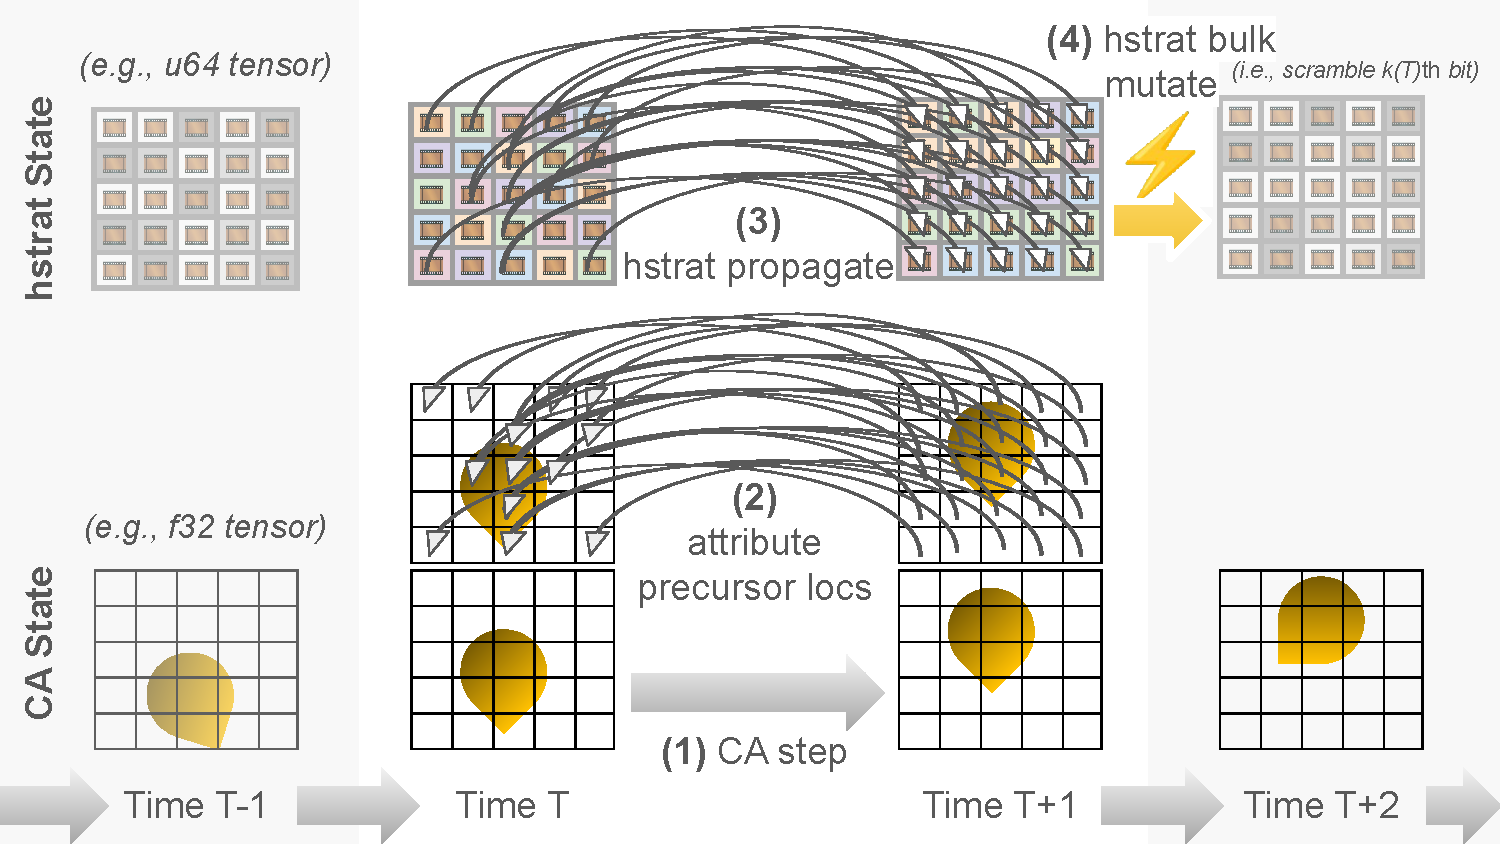
\includegraphics[width=0.8\textwidth]{img/hstrat-agentless-concept-schematic}
\caption{Proposed framework for incorporating distributed phylogeny tracking into CA systems.}
\label{fig:hstrat-agentless-concept}
\end{figure}

